\chapter{Detalles de Implementación y Experimentos}\label{chapter:implementation}

El estudio se realiz\'o en un sistema operativo Ubuntu 22.04 LTS con una CPU Intel Core i3-5020U 2.20Ghz y 12GB 1600MHz RAM. Se utiliz\'o Docker 19.03.8 para las im\'agenes de Fabric v2.4.\\

Para configurar la red se utiliz\'o Minifabric en su versi\'on m\'as reciente. Las pruebas de rendimiento se realizaron con Caliper v0.5.0 empleando el \emph{chaincode} \emph{samplecc} suministrado por Minifabric.\\

Los nodos ordenadores emplearon el mecanismo de consenso \emph{raft} en cada una de las configuraciones y los nodos pares, \emph{GoLevelDB} como base de datos de estado. Se destaca el empleo del voto por mayor\'ia en la pol\'itica de aprobaci\'on, donde todos los nodos pares fueron igualmente configurados para participar en ella. Se tuvo en cuenta el estudio en una sola organizaci\'on, pero de acuerdo a la pol\'itica de aprobaci\'on implantada, su comportamiento simula para $n$ nodos pares, una red con $n$ organizaciones de un nodo par cada una, donde se evita el sesgo que propicia la conectividad en las organizaciones y a su vez se tiene un acceso homog\'eneo de los recursos del \emph{hardware}.

\newpage
\section{Escenario de bajo volumen de transacciones}

En las tablas \ref{tab:10TPS-10BS}, \ref{tab:10TPS-50BS} y \ref{tab:10TPS-100BS} se registran los datos obtenidos para el escenario de 10 TPS.\\

\subsection{An\'alisis de latencia}
De acuerdo a los datos suministrados se puede visualizar el comportamiento de las medida de latencia para las configuraciones con diferente tama\~no en los bloques del canal.\\

\begin{figure}[htbp]
\subfigure[Tama\~no de bloque igual 10.]{
\begin{minipage}[t]{0.30\linewidth}
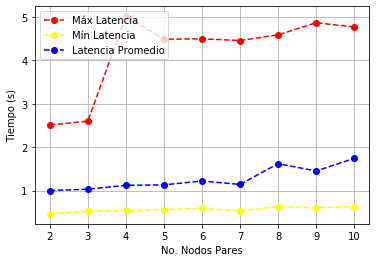
\includegraphics[scale=0.35]{Graphics/AnalisisLatenciaPares10TPSBS10.png}
\end{minipage}
}
\subfigure[Tama\~no de bloque igual 50.]{
\begin{minipage}[t]{0.30\linewidth}
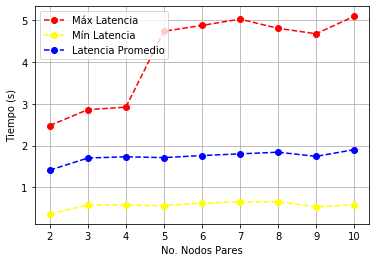
\includegraphics[scale=0.35]{Graphics/AnalisisLatenciaPares10TPSBS50.png}
\end{minipage}
}
\subfigure[Tama\~no de bloque igual 100.]{
\begin{minipage}[t]{0.30\linewidth}
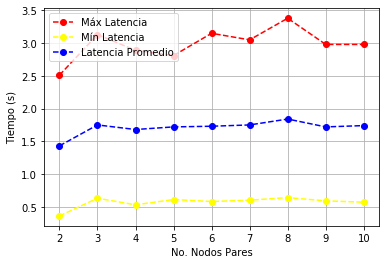
\includegraphics[scale=0.35]{Graphics/AnalisisLatenciaPares10TPSBS100.png}
\end{minipage}
}
\caption{Latencia en distintas configuraciones de nodos pares en una red con un solo nodo ordenador para escenarios de 10 TPS.}
\end{figure}

De acuerdo a la latencia m\'inima, para los tres casos mantienen un comportamiento similar, marcado por una leve tendencia al crecimiento con el aumento del n\'umero de nodos pares en la red. En el caso de la red configurada con un tama\~no de bloque igual a 10, los valores de latencia promedio son m\'as pr\'oximos a los valores de latencia m\'inima con respecto a las dem\'as configuraciones. Esto sucede porque al llegar las transacciones al servicio de ordenaci\'on, como el tama\~no del bloque es menor que el resto, y a su vez tiene una capacidad no superior al n\'umero de transacciones suministradas por los clientes, el tiempo de espera, en promedio, de las transacciones v\'alidas para cerrar el bloque es menor. Esta afirmaci\'on contrasta con la latencia m\'axima que, a menor tama\~no de bloques, mayores valores alcanza producto a que ocurre un proceso de llenado m\'as r\'apido originando una validaci\'on m\'as frecuente en los nodos pares, que a su vez participan en el proceso de simulaci\'on de las transacciones elevando la probabilidad de saturaci\'on en su proceso de ejecuci\'on.\\

En la figura \ref{ComparacionLatencia10TPS} se percibe que para un tama\~no de bloque igual a 10, el valor de latencia promedio es m\'inimo para todos las configuraciones de nodos pares. Luego, el tama\~no de bloque 10 es un par\'ametro que optimiza la latencia promedio en la red, en comparaci\'on a los dem\'as, por tanto, es un posible candidato a \'optimo.\\

\begin{figure}[h]
\centering
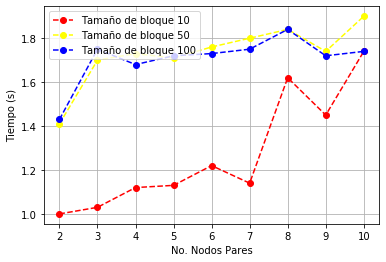
\includegraphics[scale=0.5]{Graphics/ComparacionLatencia10TPS.png}
\caption{Latencia promedio en redes con distinto tama\~no de bloque para escenarios de 10 TPS.}
\label{ComparacionLatencia10TPS}
\end{figure}


\subsection{An\'alisis de rendimiento}

\begin{figure}[h]
\subfigure[Tama\~no de bloque igual 10.]{
\begin{minipage}[t]{0.30\linewidth}
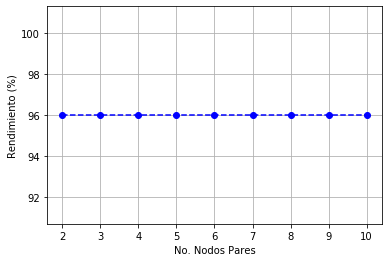
\includegraphics[scale=0.35]{Graphics/RendimientoPares10TPSBS10.png}
\end{minipage}
}
\subfigure[Tama\~no de bloque igual 50.]{
\begin{minipage}[t]{0.30\linewidth}
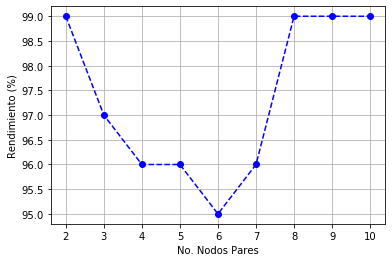
\includegraphics[scale=0.35]{Graphics/RendimientoPares10TPSBS50.png}
\end{minipage}
}
\subfigure[Tama\~no de bloque igual 100.]{
\begin{minipage}[t]{0.30\linewidth}
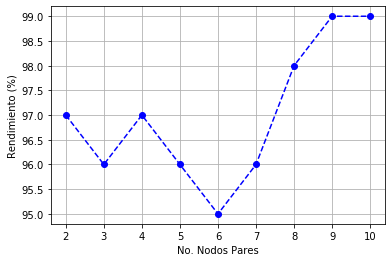
\includegraphics[scale=0.35]{Graphics/RendimientoPares10TPSBS100.png}
\end{minipage}
}
\caption{Rendimiento en distintas configuraciones de nodos pares en una red con un solo nodo ordenador para escenarios de 10 TPS.}
\end{figure}


Para los tama\~no de bloque planteados, los valores de rendimiento de la red oscilan entre el 95$\%$ y 99$\%$. La red configurada con tama\~no de bloque 10 mantiene un rendimiento constante de 96$\%$ para las configuraciones de nodos pares estudiadas.\\

 En el caso de la red con bloques de tama\~no 50 se alcanza un mejor rendimiento en la mayor\'ia de las configuraciones de nodos pares, como se puede ver en la figura \ref{RendimientoPares10TPS}.\\

\begin{figure}[h]
\centering
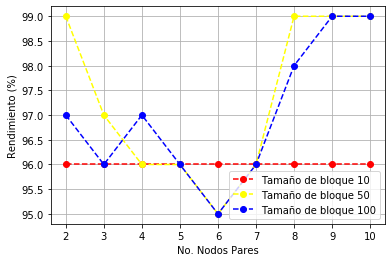
\includegraphics[scale=0.5]{Graphics/RendimientoPares10TPS.png}
\caption{Rendimiento de redes con distinto tama\~no de bloque para escenarios de 10 TPS.}
\label{RendimientoPares10TPS}
\end{figure}

\newpage

Para determinar una configuraci\'on \'optima, en relaci\'on a los valores de par\'ametros estudiados, se tuvo en cuenta el rendimiento en la red y la latencia promedio. Para establecer una comparaci\'on se llevaron las m\'etricas a una escala global, normalizando sus valores. Estos valores son estimaciones promedio para configuraciones con una cantidad de nodos pares entre dos y diez por organizaci\'on, donde el tama\~no en los bloques representa el factor a optimizar. En la figura \ref{Resultado10TPS} podemos ver que el mejor rendimiento se alcanza para canales con tama\~no de bloque igual a 50, pero a su vez la latencia promedio es mayor que la estimada para las configuraciones de canales de tama\~no 10. Por tanto, los valores 10 y 50 representan \'optimos locales, que en dependencia del escenario de uso, minimizan la latencia promedio y maximizan el rendimiento de la red respectivamente.\\

\begin{figure}[h]
\centering
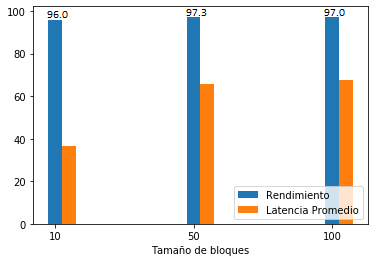
\includegraphics[scale=0.7]{Graphics/Resultado10TPS.png}
\caption{Evaluaci\'on de resultados para escenarios de 10 TPS.}
\label{Resultado10TPS}
\end{figure}

\newpage

\section{Escenario de alto volumen de transacciones}

En las tablas \ref{tab:100TPS-10BS}, \ref{tab:100TPS-50BS} y \ref{tab:100TPS-100BS} se registran los datos obtenidos para el escenario de 100 TPS.\\

\subsection{An\'alisis de latencia}

Las siguientes gr\'aficas muestran el comportamiento de la latencia promedio en la red configurada con cada tama\~no de bloque estudiado.\\

\begin{figure}[htbp]
\subfigure[Tama\~no de bloque igual 10.]{
\begin{minipage}[t]{0.30\linewidth}
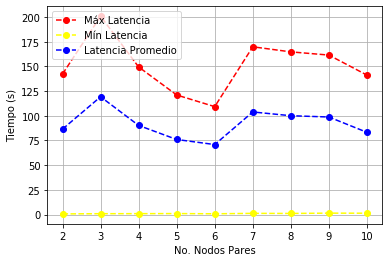
\includegraphics[scale=0.35]{Graphics/AnalisisLatenciaPares100TPSBS10.png}
\end{minipage}
}
\subfigure[Tama\~no de bloque igual 50.]{
\begin{minipage}[t]{0.30\linewidth}
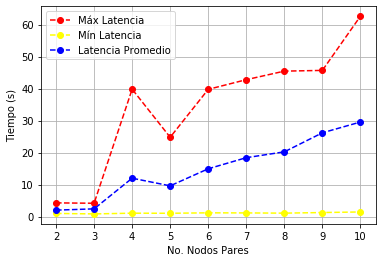
\includegraphics[scale=0.35]{Graphics/AnalisisLatenciaPares100TPSBS50.png}
\end{minipage}
}
\subfigure[Tama\~no de bloque igual 100.]{
\begin{minipage}[t]{0.30\linewidth}
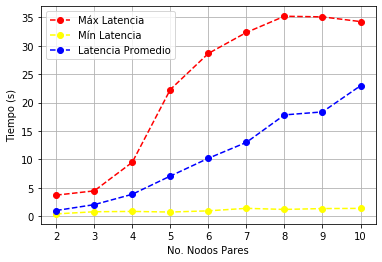
\includegraphics[scale=0.35]{Graphics/AnalisisLatenciaPares100TPSBS100.png}
\end{minipage}
}
\caption{Latencia en distintas configuraciones de nodos pares en una red con un solo nodo ordenador para escenarios de 100 TPS.}
\end{figure}


En la primera gr\'afica podemos observar que los valores de latencia promedio oscilan entre los 70 y 120 segundos aproximadamente. Estos valores son, en extremo, elevados en comparaci\'on con las restantes configuraciones. Para el caso de los bloques de tama\~no 100 el mayor valor alcanzado de latencia promedio, no supera los 25 segundos, quedando todos sus valores por debajo de los alcanzados por la configuraci\'on de bloques de tama\~no 10. Lo mismo sucede en las redes con bloques de tama\~no 50 que no superan los 30 segundos.\\

Para determinar el tama\~no de bloque que ofrece mejor desempe\~no en redes con un n\'umero de nodos pares que var\'ia de dos a diez por organizaci\'on,  con respecto a la latencia de las transacciones, se calcul\'o la media de las latencias promedios de las configuraciones de nodos pares, por tama\~nos de bloques, y nos quedamos con la configuraci\'on de bloque que corresponda a la menor de ellas.\\

Los bloques de tama\~no 10, 50 y 100 promedian una latencia media para las configuraciones de nodos pares de 92.1, 15.0 y 10.7 segundos respectivamente. Por tanto, las redes configuradas con bloques de tama\~no 100 son \'optimas respecto al conjunto estudiado, propiciando la menor latencia promedio. Para establecer una comparativa visual nos podemos remitir a la figura \ref{ComparacionLatencia100TPS}.\\

\begin{figure}[h]
\centering
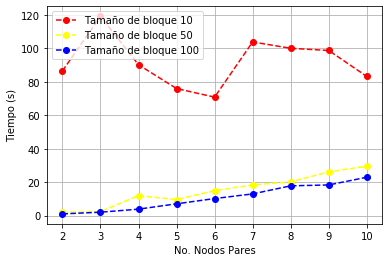
\includegraphics[scale=0.5]{Graphics/ComparacionLatencia100TPS.png}
\caption{Latencia promedio en redes con distinto tama\~no de bloque para escenarios de 100 TPS.}
\label{ComparacionLatencia100TPS}
\end{figure}

\subsection{An\'alisis de rendimiento}

\begin{figure}[h]
\subfigure[Tama\~no de bloque igual 10.]{
\begin{minipage}[t]{0.30\linewidth}
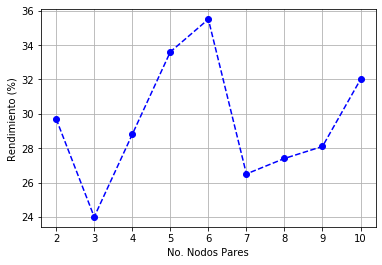
\includegraphics[scale=0.35]{Graphics/RendimientoPares100TPSBS10.png}
\end{minipage}
}
\subfigure[Tama\~no de bloque igual 50.]{
\begin{minipage}[t]{0.30\linewidth}
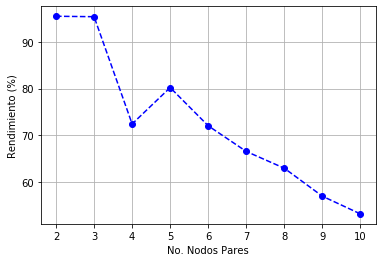
\includegraphics[scale=0.35]{Graphics/RendimientoPares100TPSBS50.png}
\end{minipage}
}
\subfigure[Tama\~no de bloque igual 100.]{
\begin{minipage}[t]{0.30\linewidth}
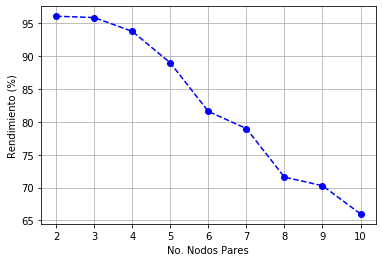
\includegraphics[scale=0.35]{Graphics/RendimientoPares100TPSBS100.png}
\end{minipage}
}
\caption{Rendimiento en distintas configuraciones de nodos pares en una red con un solo nodo ordenador para escenarios de 100 TPS.}
\end{figure}

De acuerdo a la gr\'afica que representa el rendimiento para las redes con bloques de tama\~no 10, se destaca el bajo rendimiento que logran en escenarios de altos vol\'umenes de transacciones. Entre las causas fundamentales que lo ocasionan est\'a el r\'apido llenado de los bloques por el servicio de ordenaci\'on, que luego son enviados, con mayor frecuencia, a los nodos pares para el proceso de validaci\'on y a su vez se conjuga con el alto volumen de transacciones que deben simular en cada intervalo de tiempo. Los bloques de tama\~no 50 y 100 manifiestan un mejor rendimiento debido a que compensan la frecuencia de validaci\'on por los nodos pares, con un aumento del tiempo de conformaci\'on de bloques.\\

Si ilustramos las curvas de rendimiento en una sola gr\'afica, como en la figura \ref{RendimientoPares100TPS}, apreciamos que las redes con bloques de tama\~no 100 superan para todas las configuraciones de nodos pares, a las redes con bloques de tama\~no inferior. Se aprecia adem\'as, que para escenarios de altos vol\'umenes de transacciones por segundo, el aumento del n\'umero de nodos pares en las organizaciones reducen el rendimiento de forma considerable.

\begin{figure}[h]
\centering
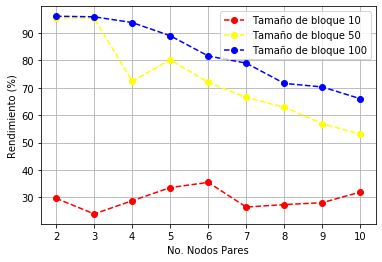
\includegraphics[scale=0.5]{Graphics/RendimientoPares100TPS.png}
\caption{Rendimiento de redes con distinto tama\~no de bloque para escenarios de 100 TPS.}
\label{RendimientoPares100TPS}
\end{figure}

En este escenario, la configuraci\'on para bloques de tama\~no 100, propicia la menor latencia promedio en la red y el mejor desempe\~no en el rendimiento, del conjunto evaluado. En la figura \ref{Resultado100TPS} se puede ver el marcado contraste dado por la diferencia en el tama\~no de los bloques. Se tiene una diferencia m\'axima de latencia superior a los 80 segundos, igual comportamiento tenemos en el rendimiento, donde los bloque de tama\~no 10 ofrecen las m\'etricas m\'as desfavorables. A su vez, esta coincide con la configuraci\'on, por defecto, de la red para los canales de comunicaci\'on. Por tanto, confirma la necesidad de evaluar los par\'ametros del sistema antes de su puesta en producci\'on.\\

\begin{figure}[h]
\centering
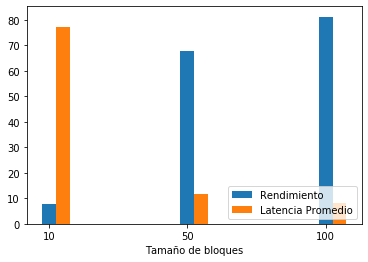
\includegraphics[scale=0.6]{Graphics/Resultado100TPS.png}
\caption{Evaluaci\'on de resultados para escenarios de 100 TPS.}
\label{Resultado100TPS}
\end{figure}

%\section*{An\'alisis de la influencia de los nodos pares y ordenadores en los escenarios estudiados}
